\subparagraph{Sensitivity estimate}

\begin{figure}[tbp]
\centering
\begin{subfigure}{0.48\textwidth}
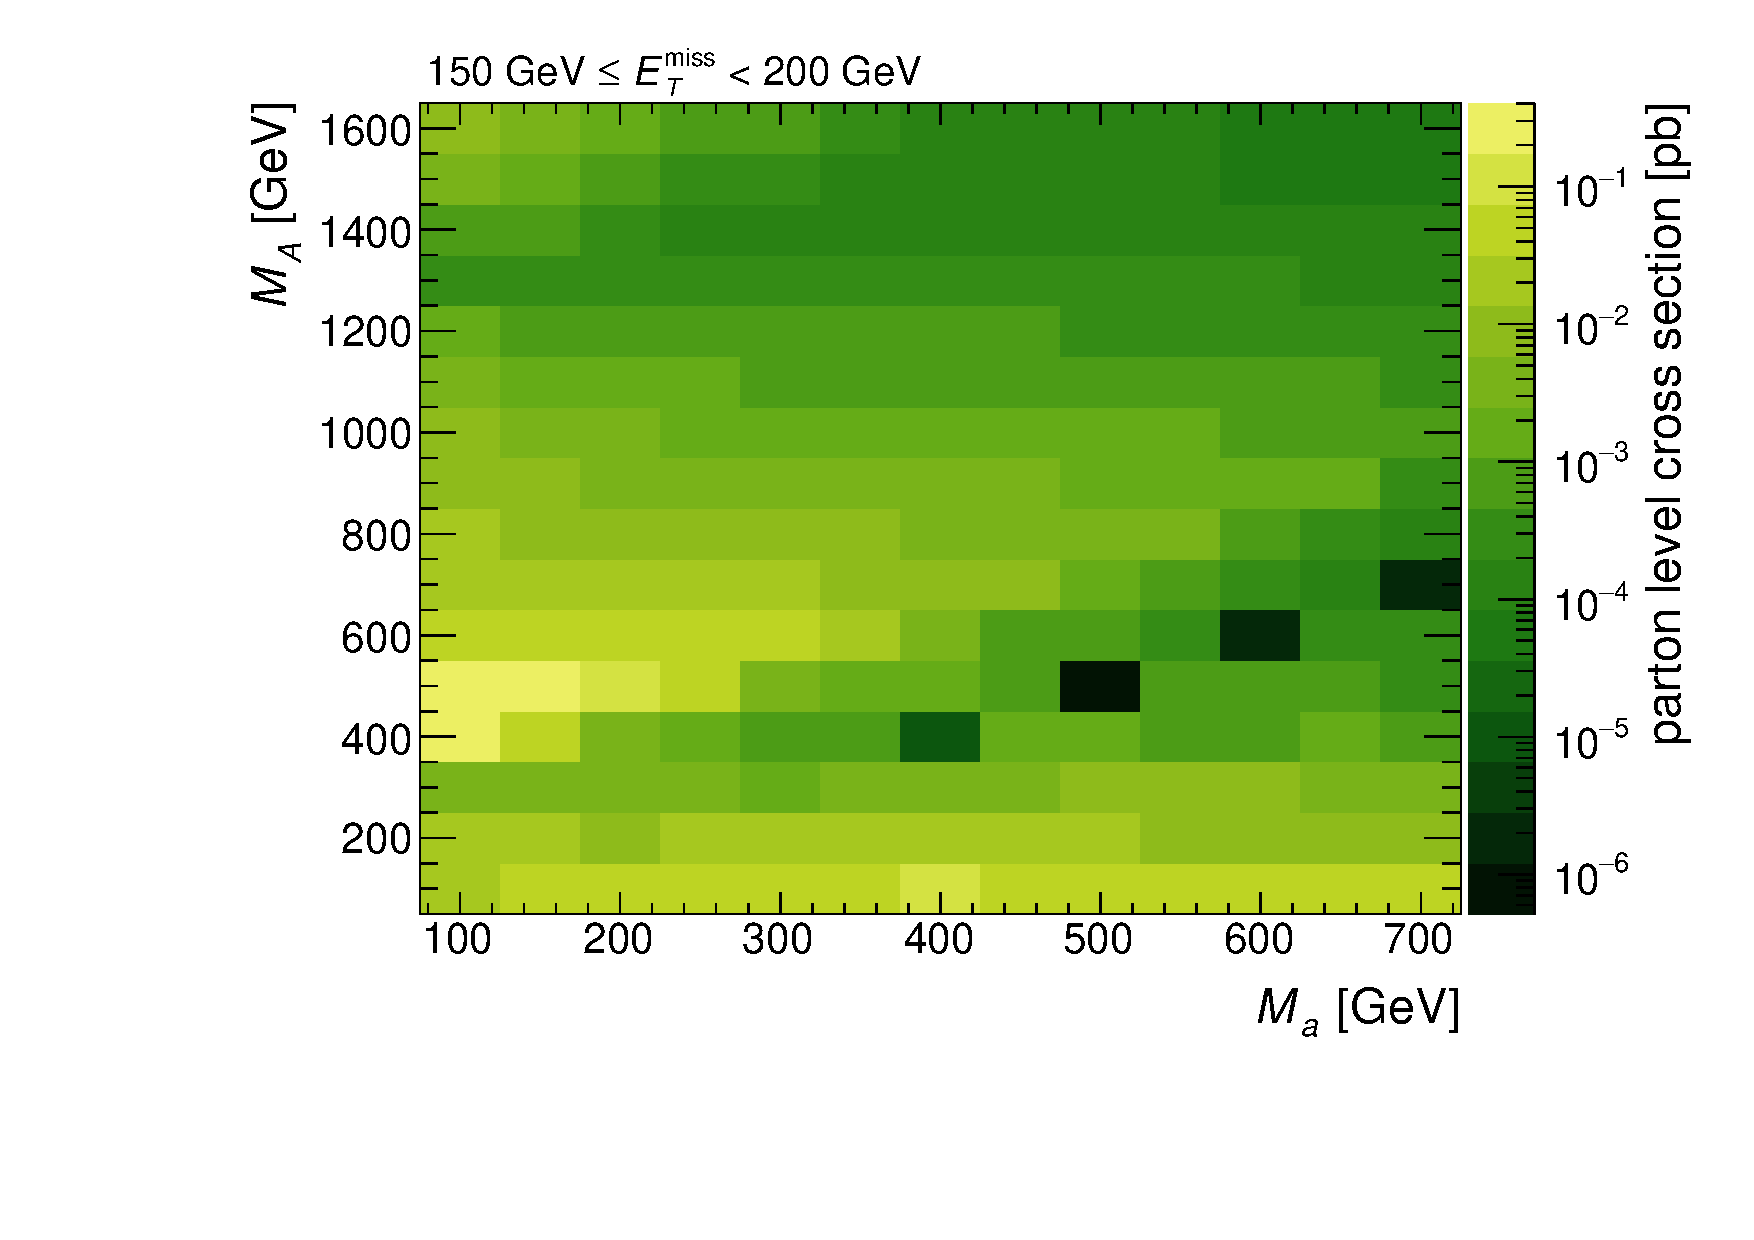
\includegraphics[width = \textwidth]{texinputs/04_grid/figures/monoHbb_parton_level_cross_section_bin_1_ma_vs_mA_lin.pdf}
\end{subfigure}
~
\begin{subfigure}{0.48\textwidth}
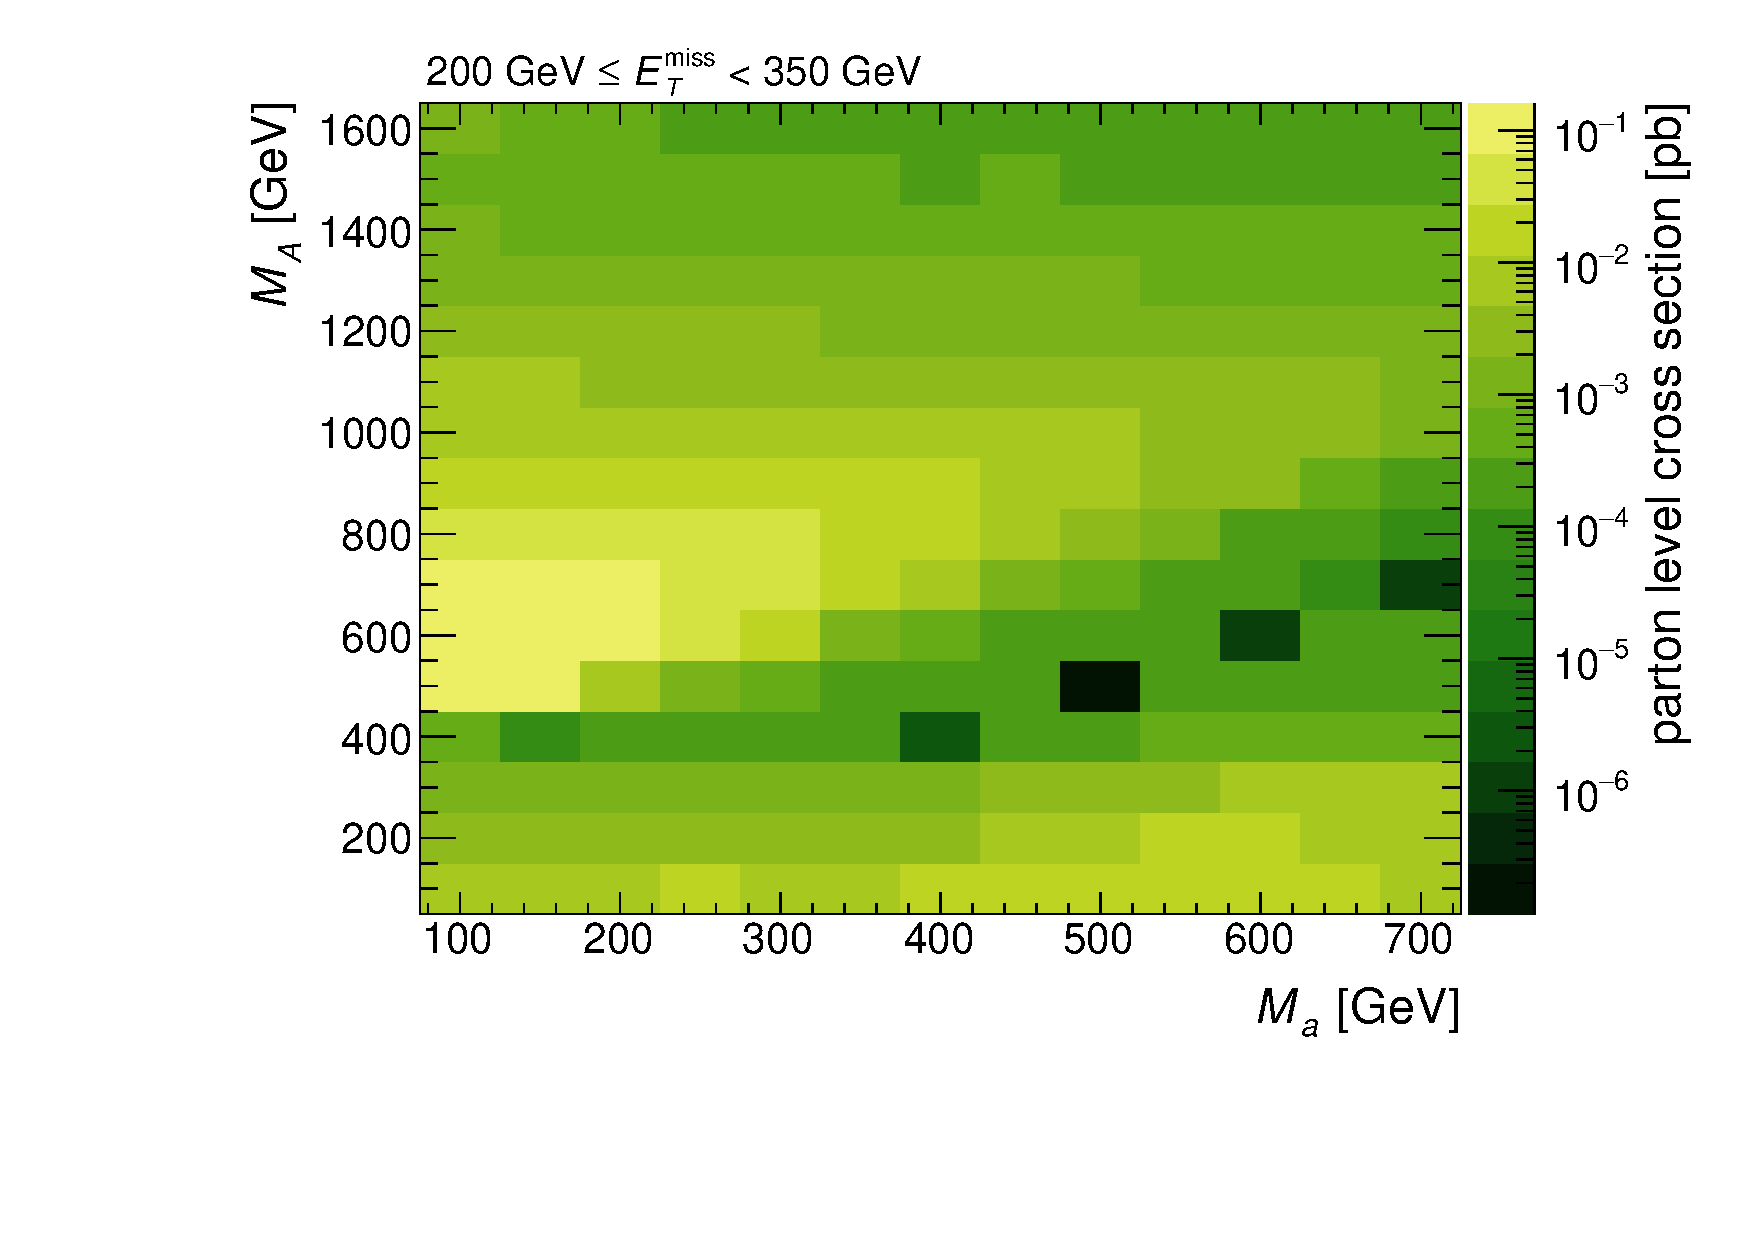
\includegraphics[width = \textwidth]{texinputs/04_grid/figures/monoHbb_parton_level_cross_section_bin_2_ma_vs_mA_lin.pdf}
\end{subfigure}
\\
\centering
\begin{subfigure}{0.48\textwidth}
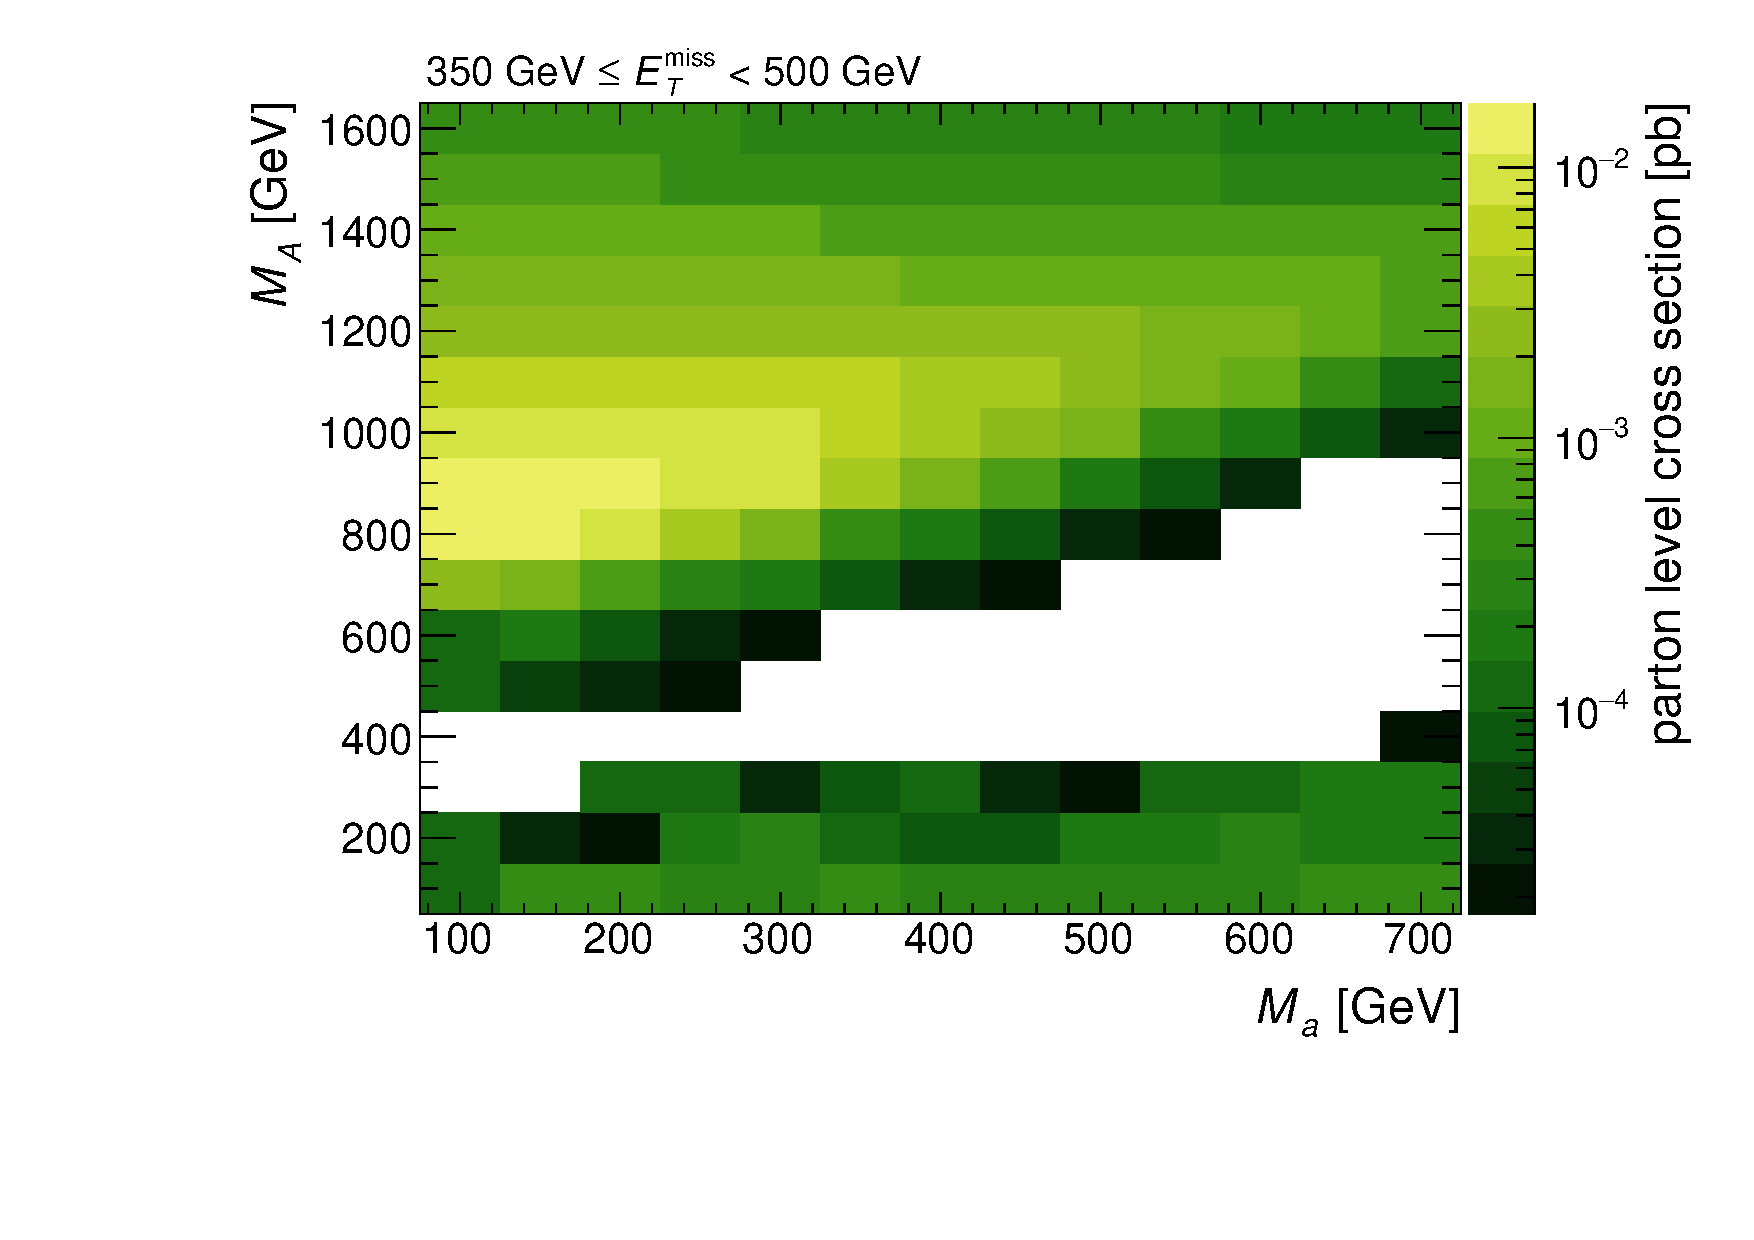
\includegraphics[width = \textwidth]{texinputs/04_grid/figures/monoHbb_parton_level_cross_section_bin_3_ma_vs_mA_lin.pdf}
\end{subfigure}
~
\begin{subfigure}{0.48\textwidth}
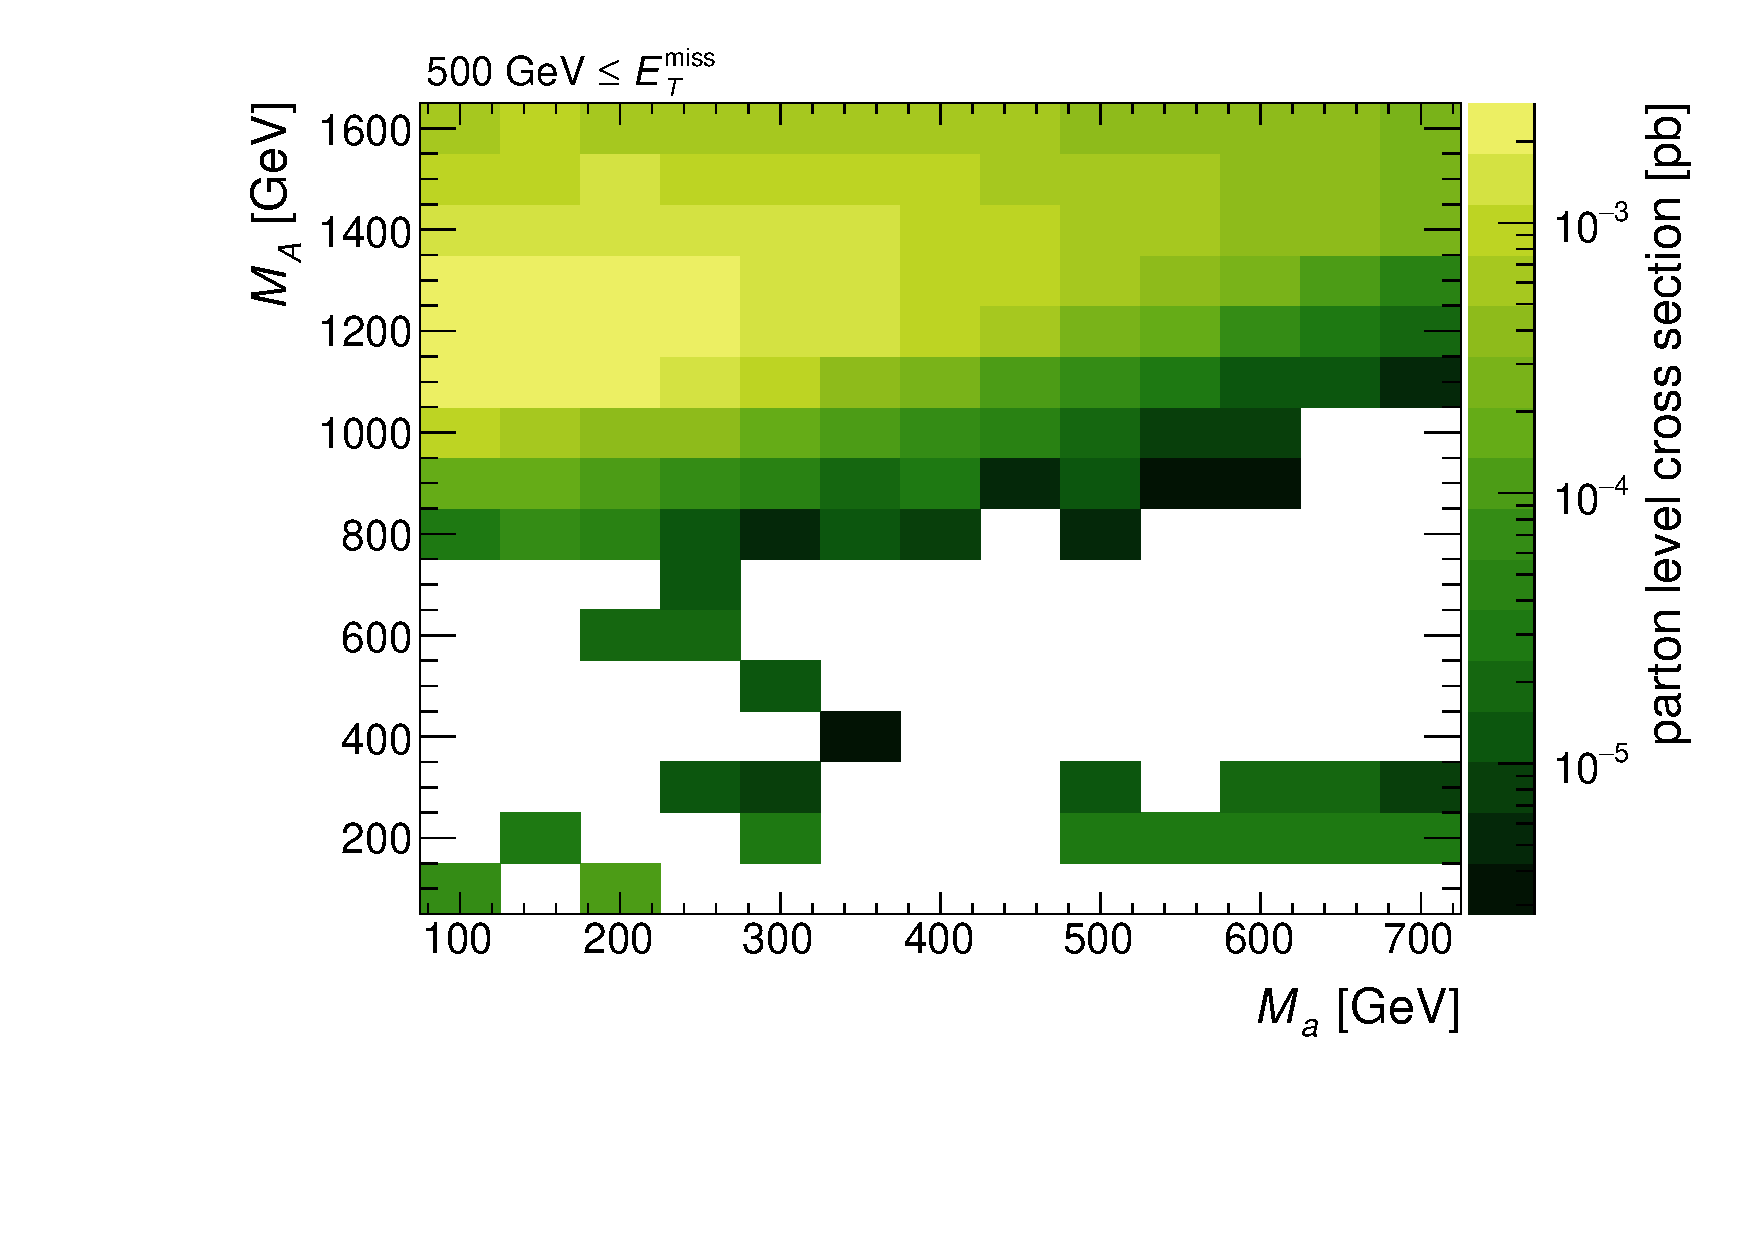
\includegraphics[width = \textwidth]{texinputs/04_grid/figures/monoHbb_parton_level_cross_section_bin_4_ma_vs_mA_lin.pdf}
\end{subfigure}
\caption[$h\to bb + \MET$ cross section binned in $\MET$, $\mA$ - $\ma$ plane ]
{
The production cross section of $h\to bb + \MET$ signal events at parton level as a function of $(\mA,\ma)$ in each of the four \met bins. 
The remaining parameters take the values
$ \mH=\mHc= \mA, \sinp = 0.35, \tanb = 1, \mDM = 10$ GeV and $ \lap1 = \lap2 = \lam3 = 3 $.
}
\label{fig:monoHbb_xsec_bins_mA_ma}
\end{figure}

\begin{figure}[tbp]
\centering
\begin{subfigure}{0.48\textwidth}
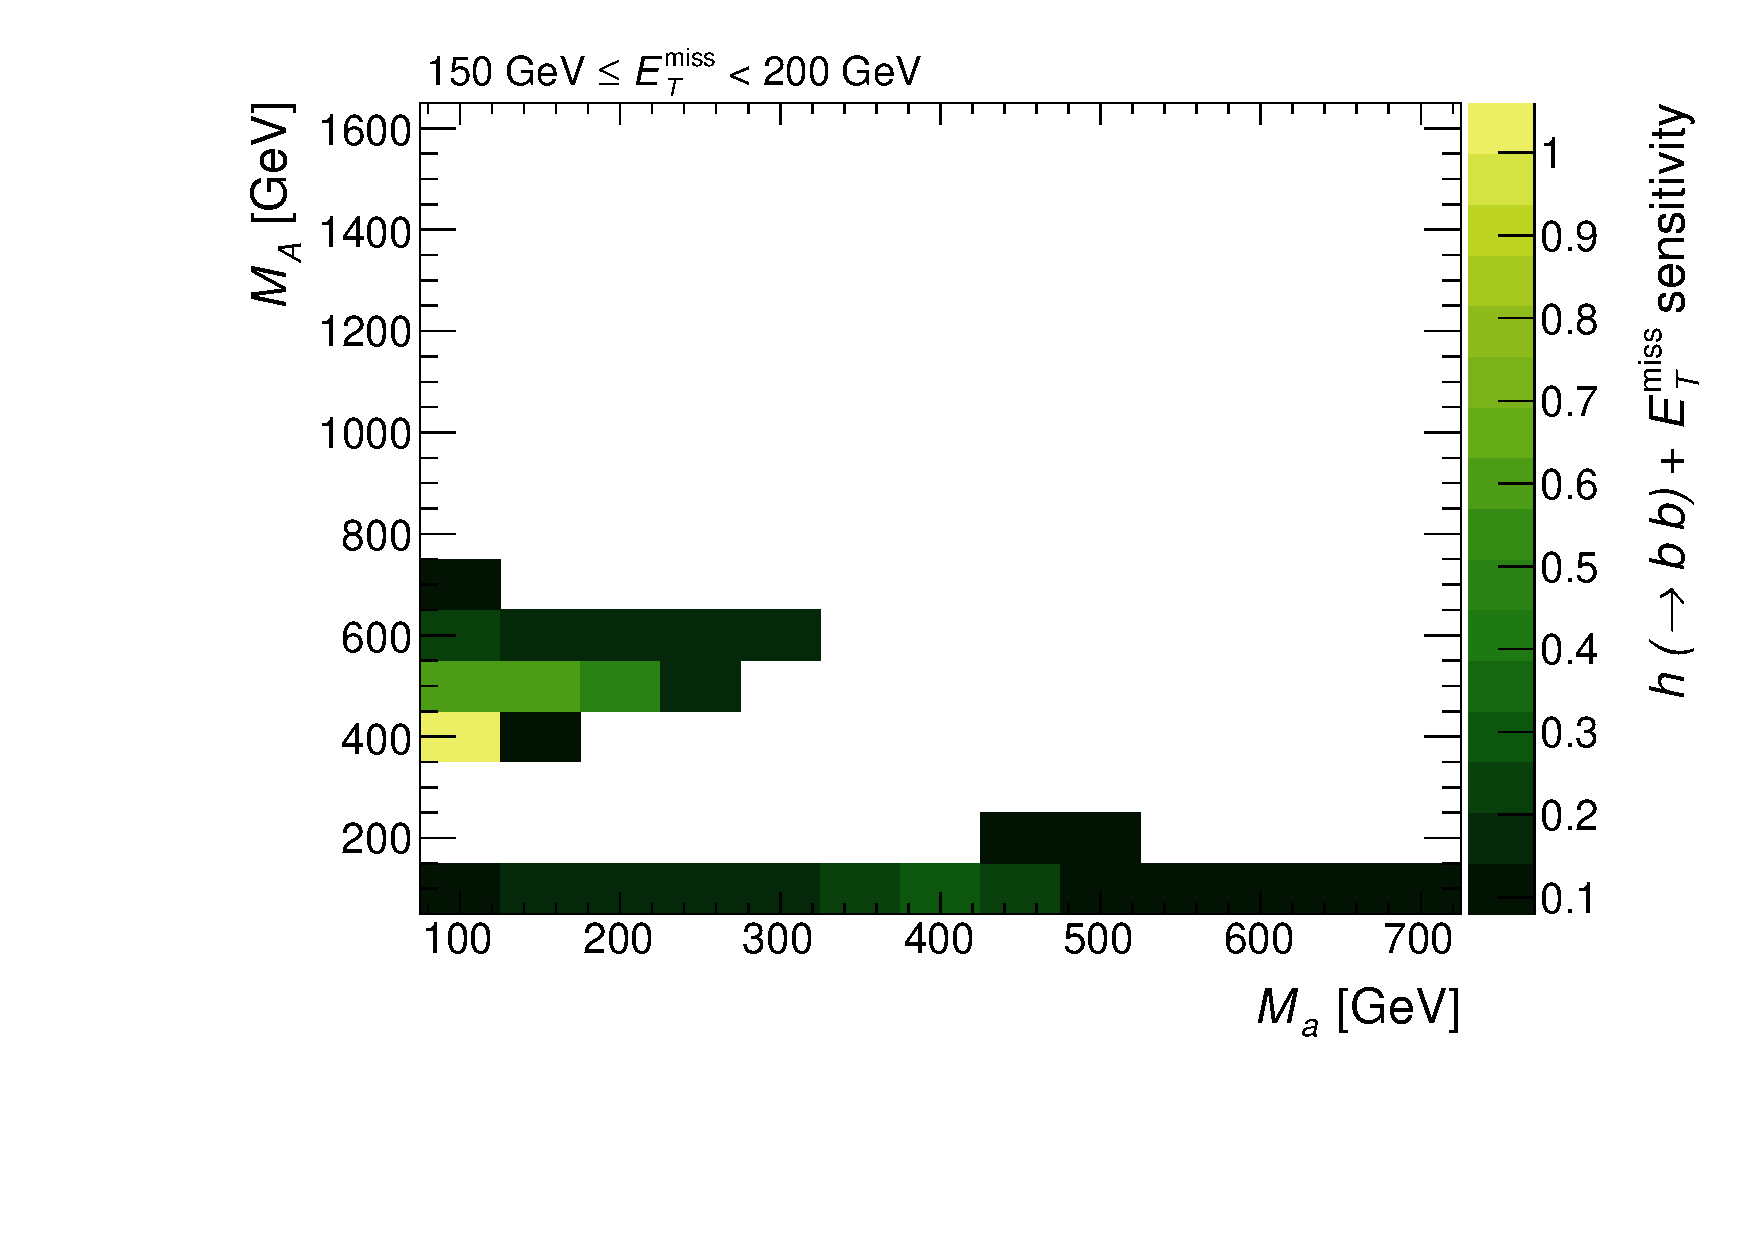
\includegraphics[width = \textwidth]{texinputs/04_grid/figures/monoHbb_sensi_bin_1_ma_vs_mA_lin.pdf}
\end{subfigure}
~
\begin{subfigure}{0.48\textwidth}
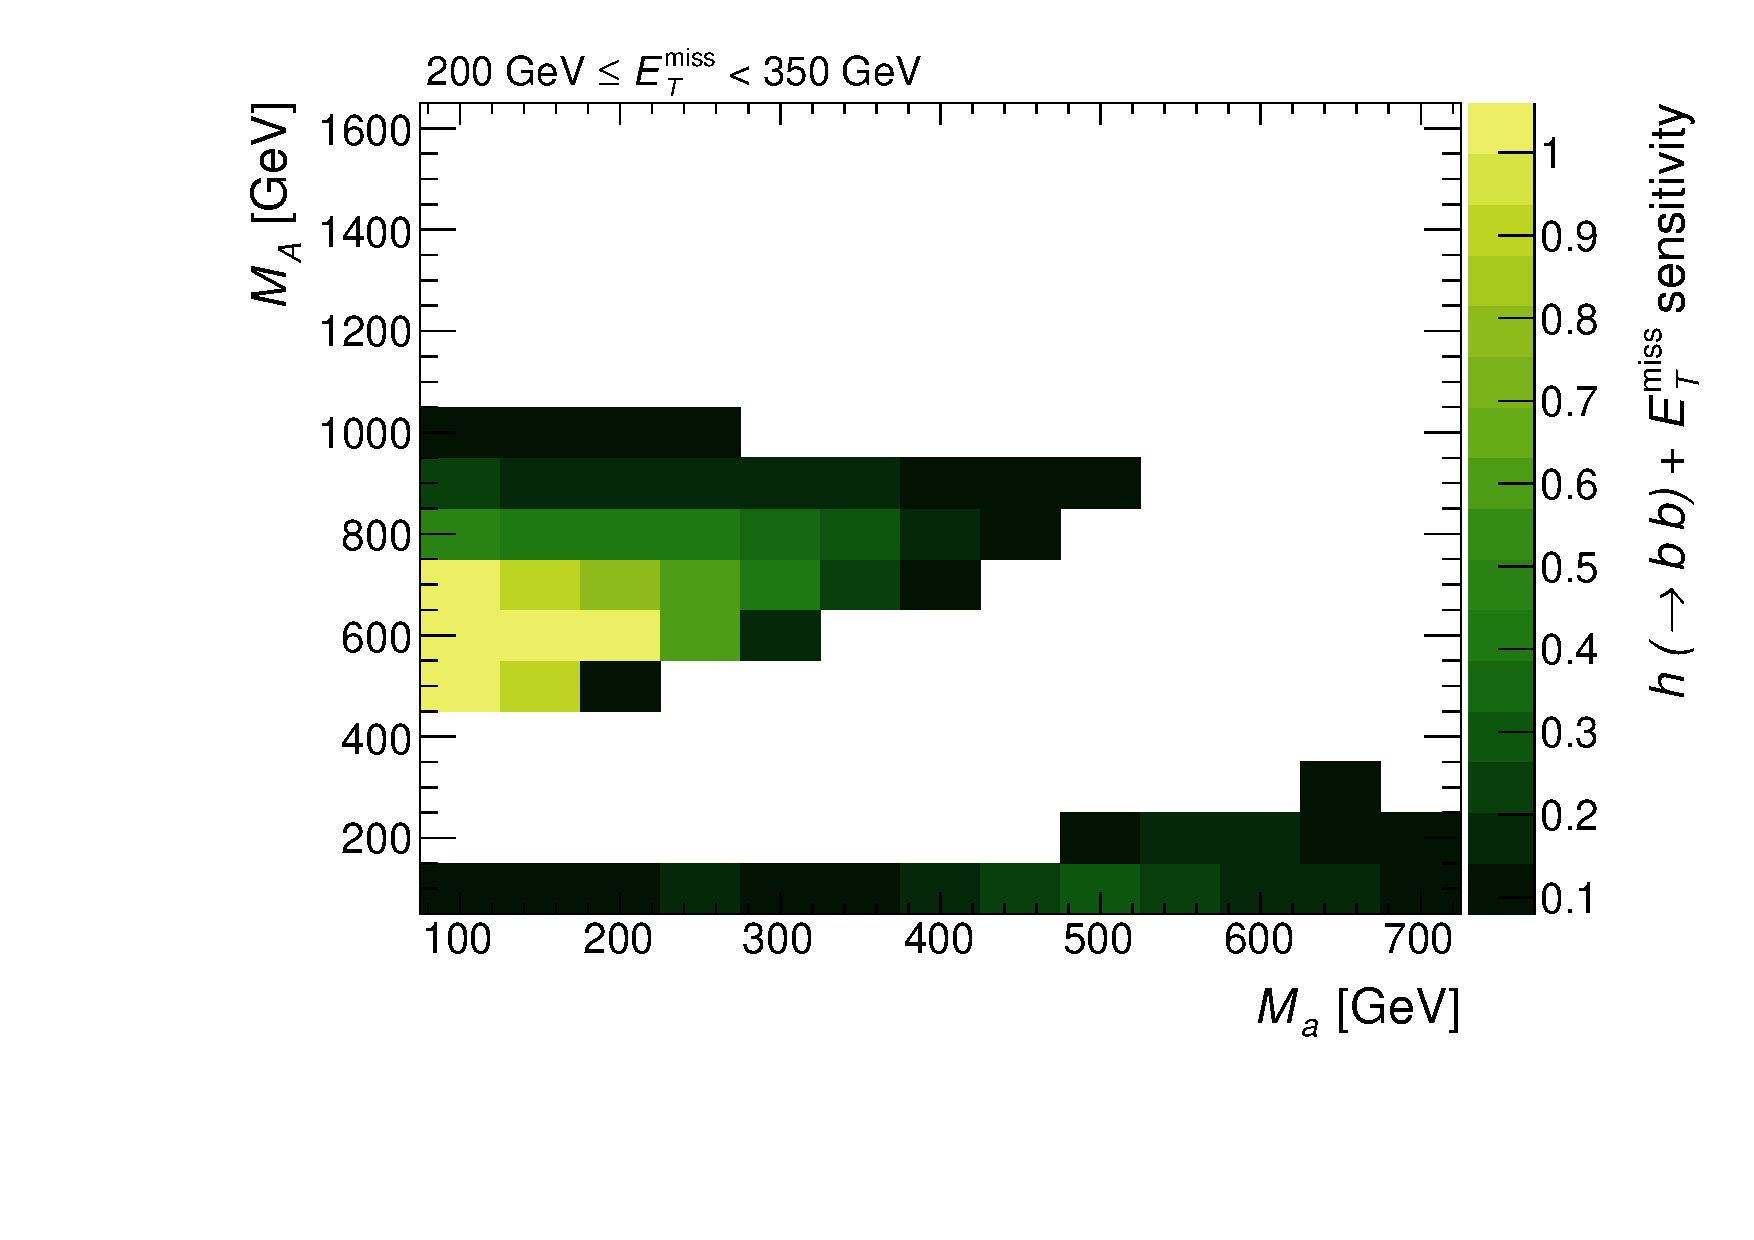
\includegraphics[width = \textwidth]{texinputs/04_grid/figures/monoHbb_sensi_bin_2_ma_vs_mA_lin.pdf}
\end{subfigure}
\\
\centering
\begin{subfigure}{0.48\textwidth}
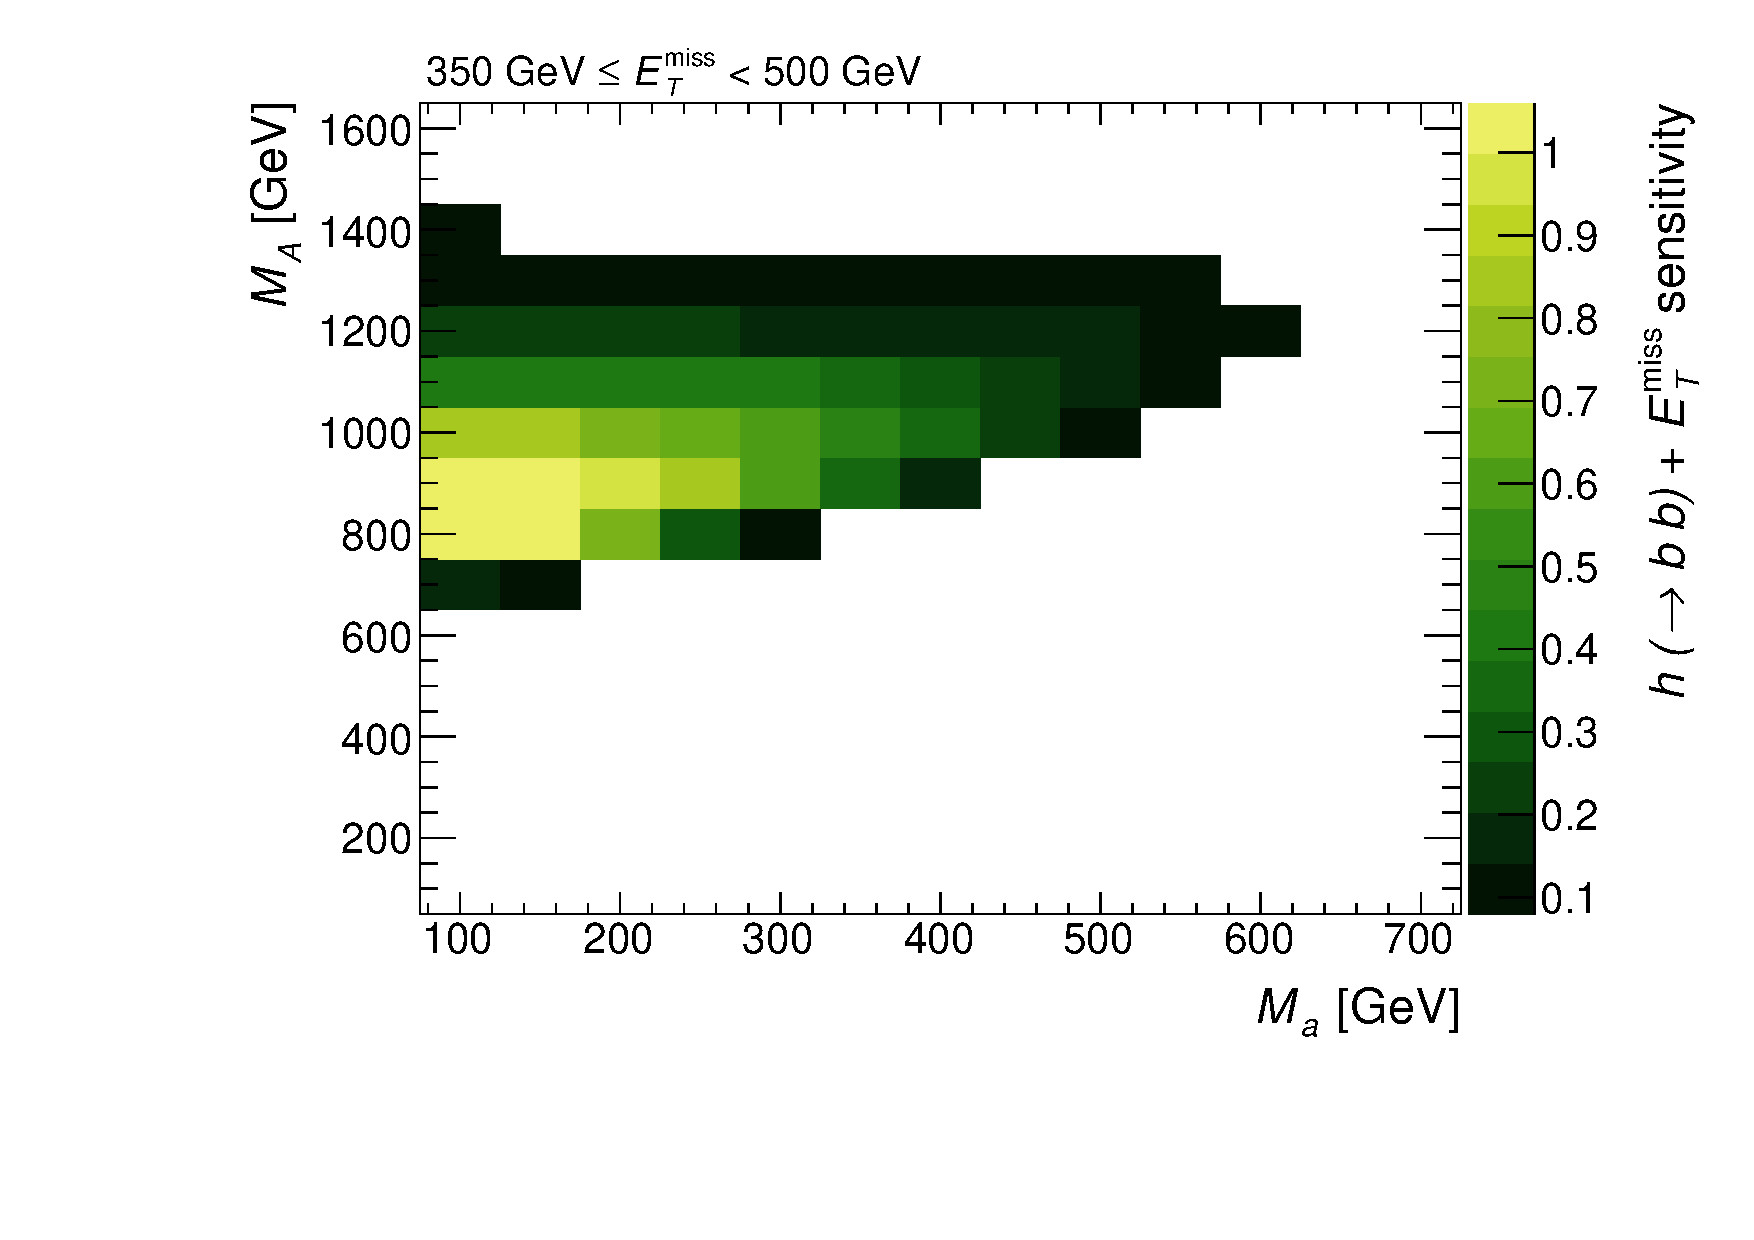
\includegraphics[width = \textwidth]{texinputs/04_grid/figures/monoHbb_sensi_bin_3_ma_vs_mA_lin.pdf}
\end{subfigure}
~
\begin{subfigure}{0.48\textwidth}
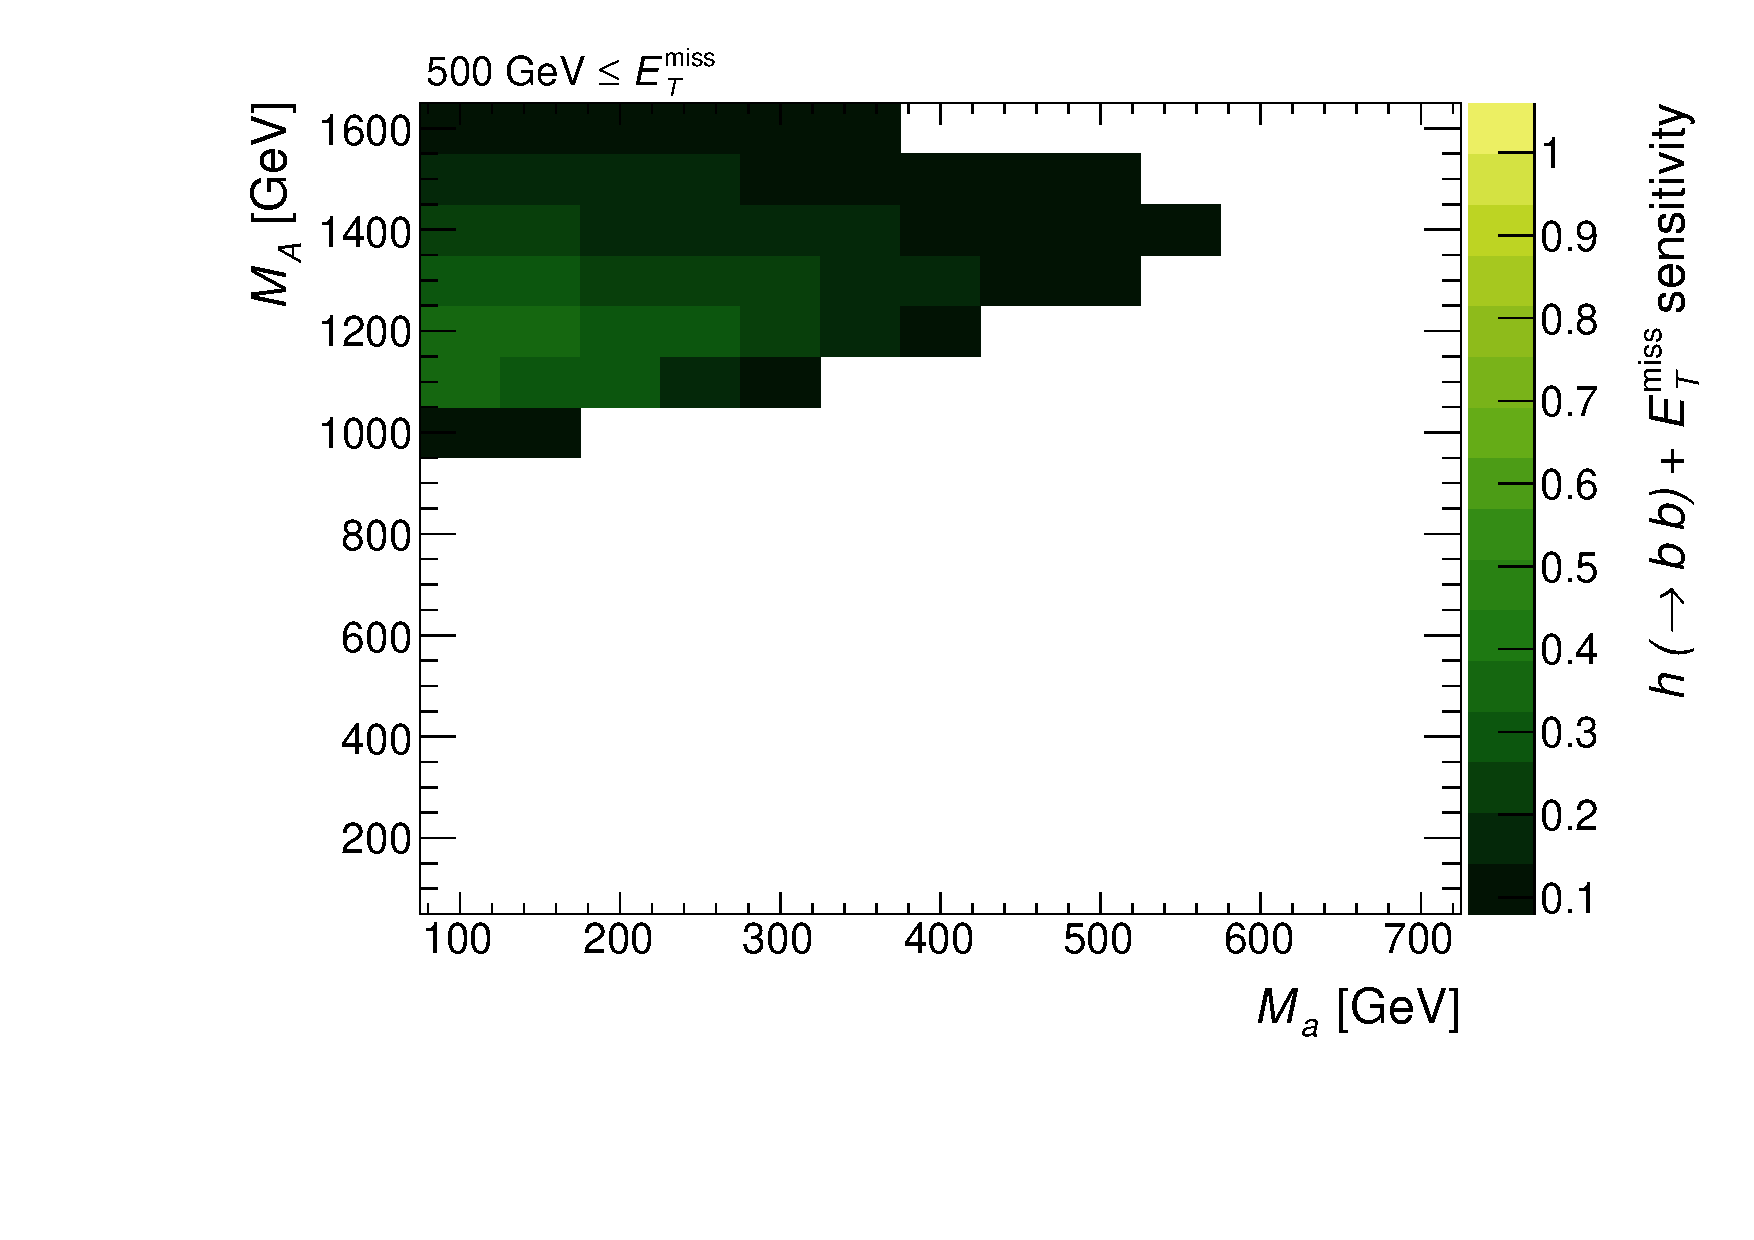
\includegraphics[width = \textwidth]{texinputs/04_grid/figures/monoHbb_sensi_bin_4_ma_vs_mA_lin.pdf}
\end{subfigure}
\caption[Sensitivity to the $h\to bb + \MET$ signal by $\MET$ bin, $\mA$ - $\ma$ plane]
{Estimated sensitivity to $h\to bb + \MET$ events as a function of $(\mA,\ma)$ in each of  the four \met bins. 
The sensitivity, defined in \autoref{eq:monoHbb_sensi}, is based on the limits with reduced model dependence from Ref.~\cite{Aaboud:2017yqz}. 
The remaining parameters take the values
$ \mH=\mHc= \mA, \sinp = 0.35, \tanb = 1, \mDM = 10$ GeV and $ \lap1 = \lap2 = \lam3 = 3 $.}
\label{fig:monoHbb_sensi_bins_mA_ma}
\end{figure}

%\begin{figure}[tbp]
%\centering
%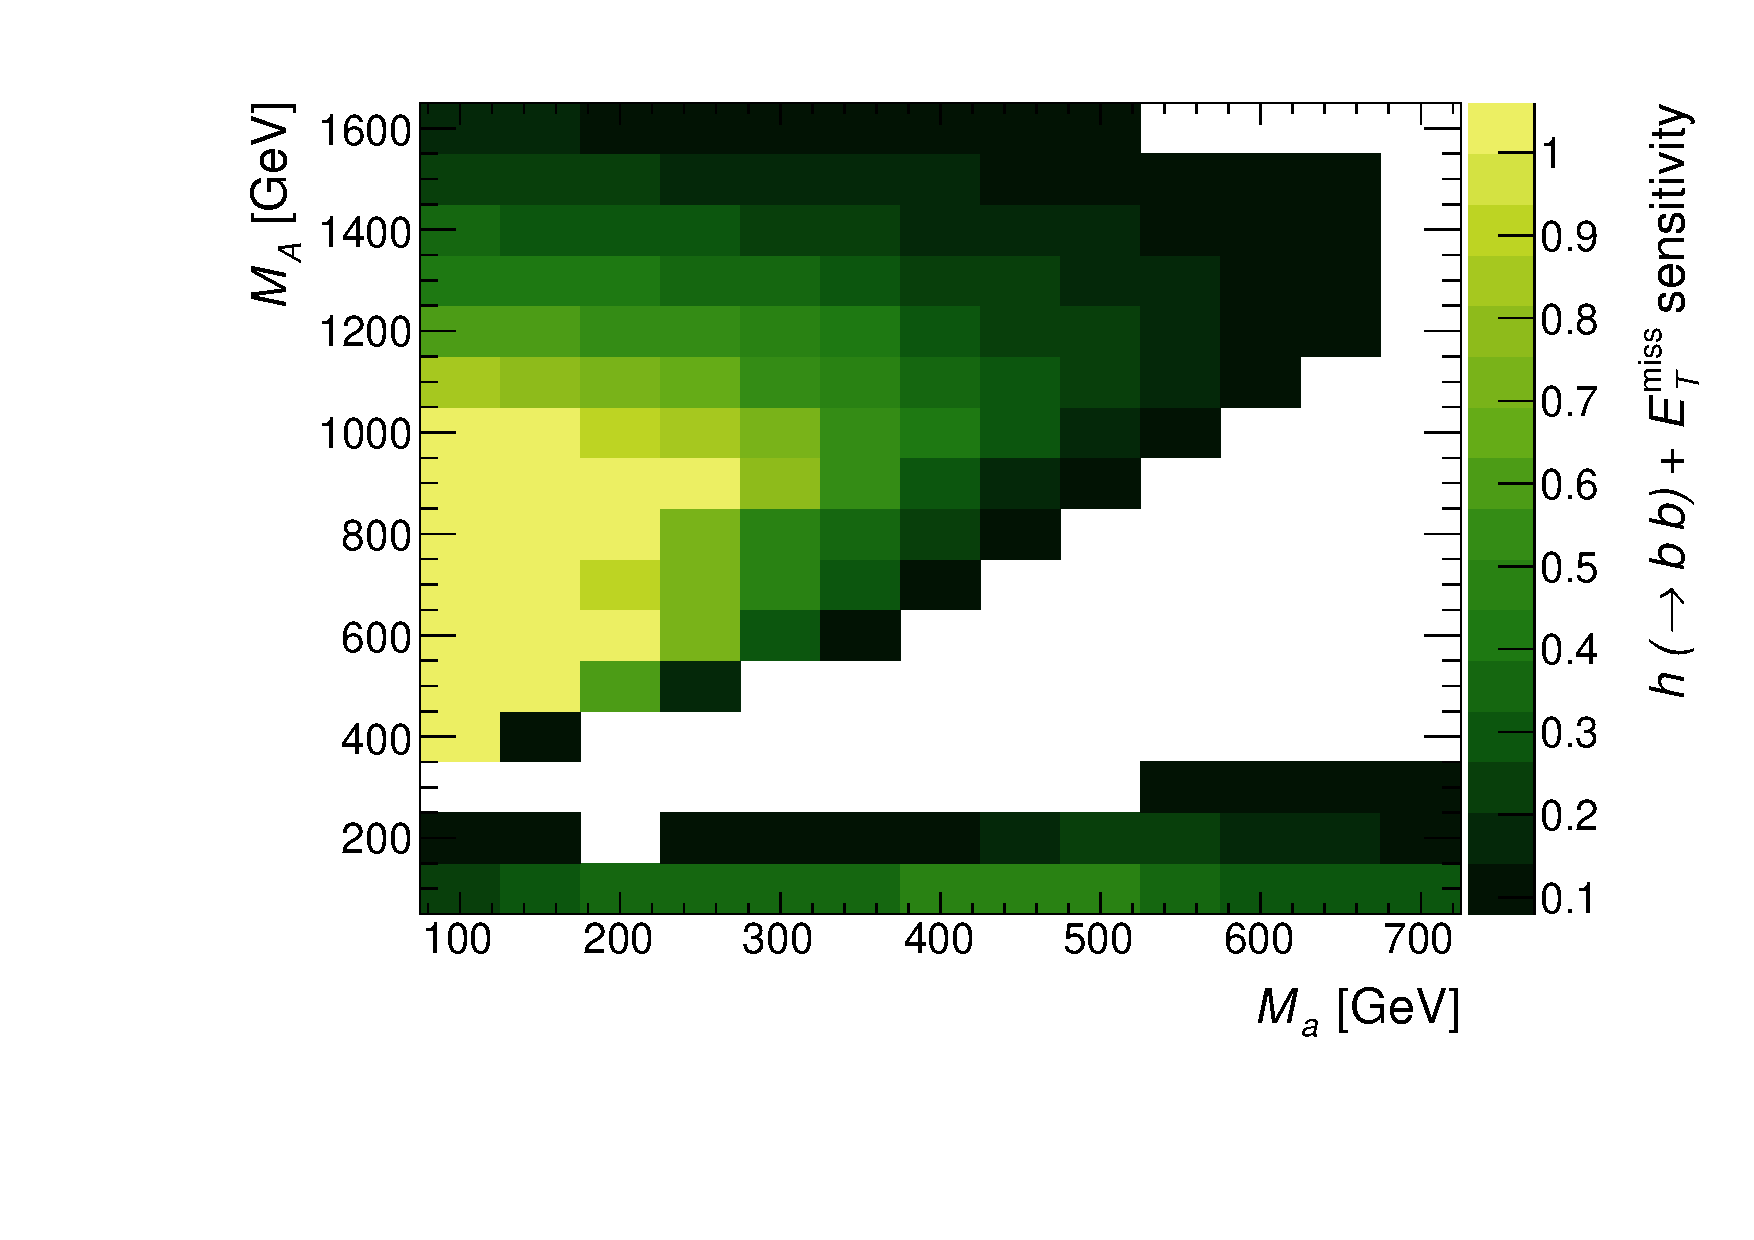
\includegraphics[width=0.7\textwidth]{texinputs/04_grid/figures/monoHbb_sensi_sum_bins_1_2_3_4_ma_vs_mA_lin.pdf}
%\caption[Sensitivity to $h\to bb + \MET$ signals in $\mA$ - $\ma$ plane, summed across $\MET$ bins]
%{
%Sum over all $\MET$-bins of the estimated sensitivity to $h\to bb + \MET$ events as a function of $(\mA,\ma)$. 
%The sensitivity, defined in \autoref{eq:monoHbb_sensi}, is based on the limits with reduced model dependence from Ref.~\cite{Aaboud:2017yqz}. 
%The remaining parameters take the values $ \mH=\mHc= \mA, \sinp = 0.35, \tanb = 1, \mDM = 10$ GeV and $ \lap1 = \lap2 = \lam3 = 3 $.}
%\label{fig:monoHbb_sensi_full_mA_ma}
%\end{figure}

%
%\begin{figure}[tbp]
%\centering
%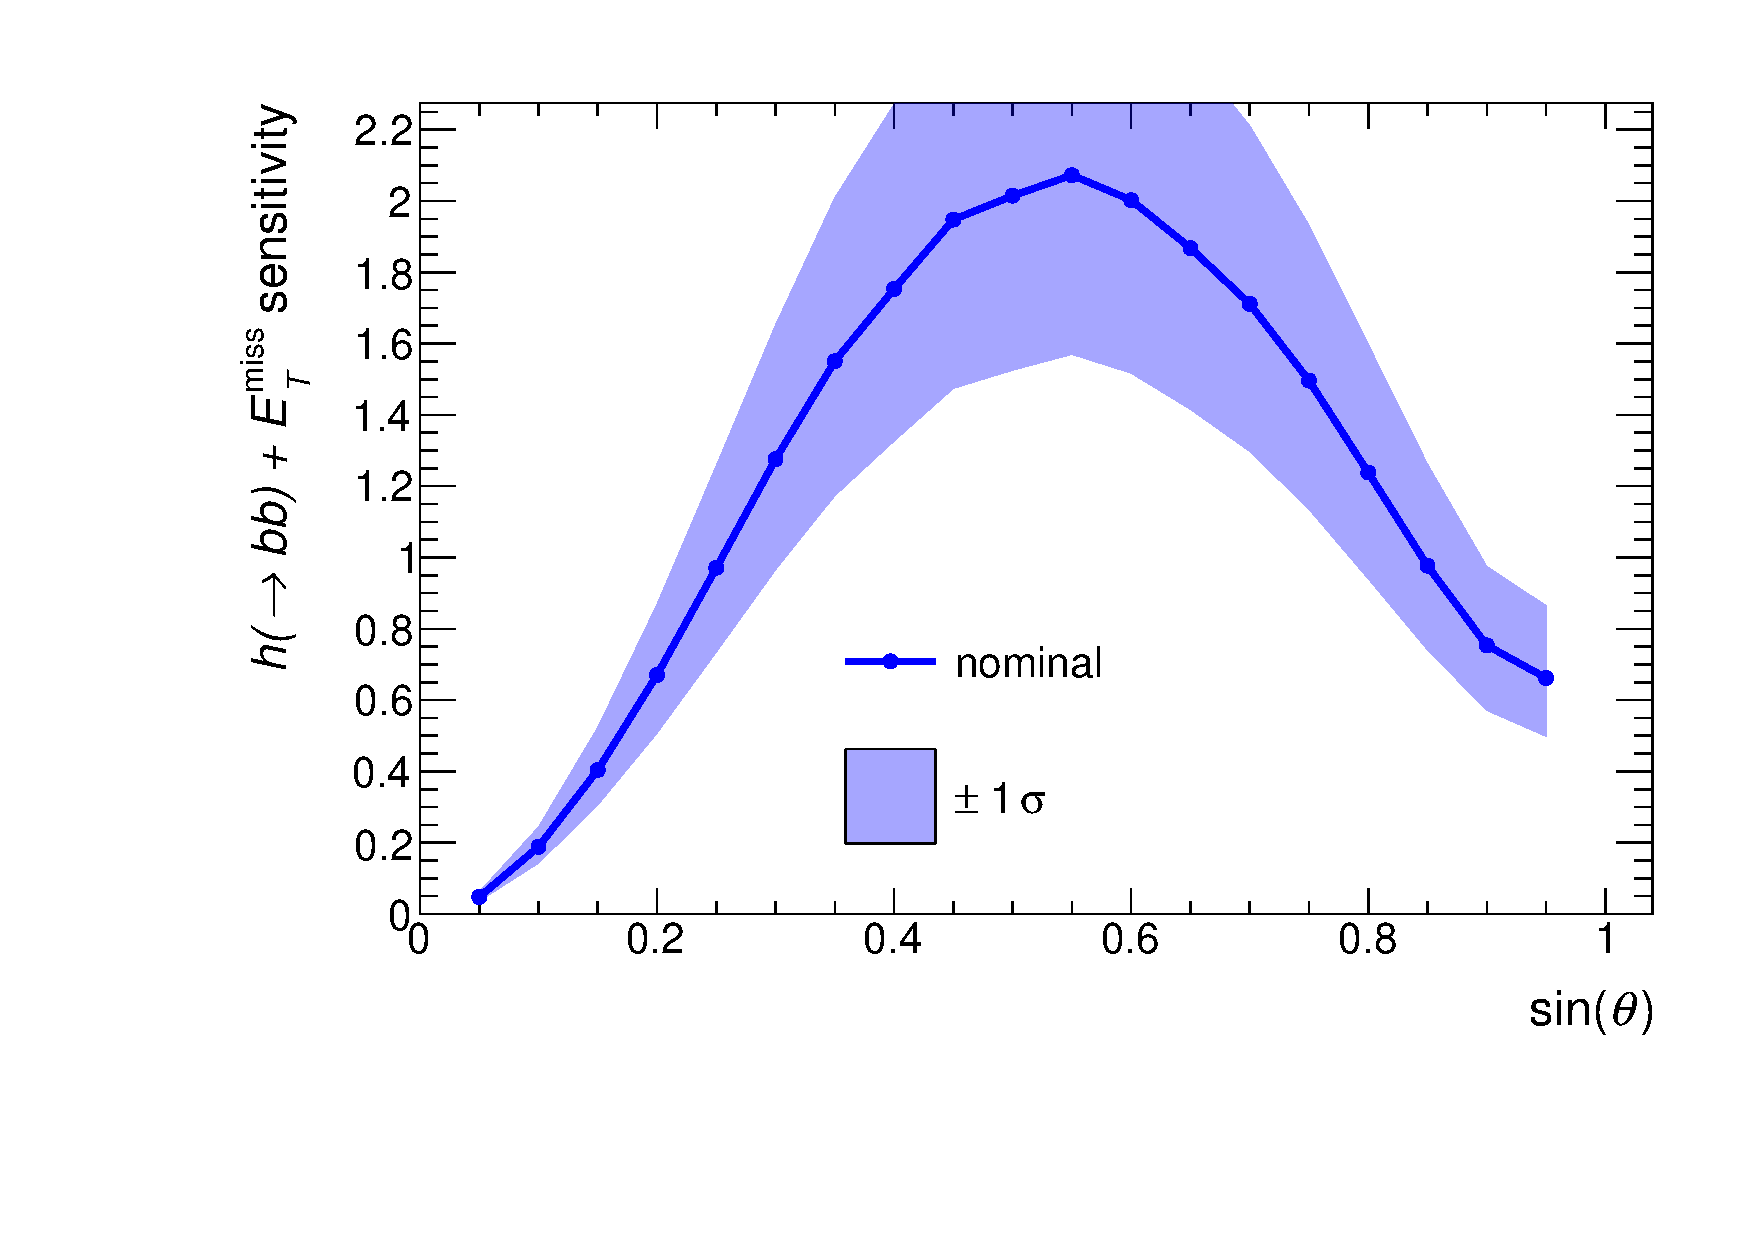
\includegraphics[width=0.49\textwidth]{texinputs/04_grid/figures/monoHbb_sinp_scan_1_sensi_1D.pdf}
%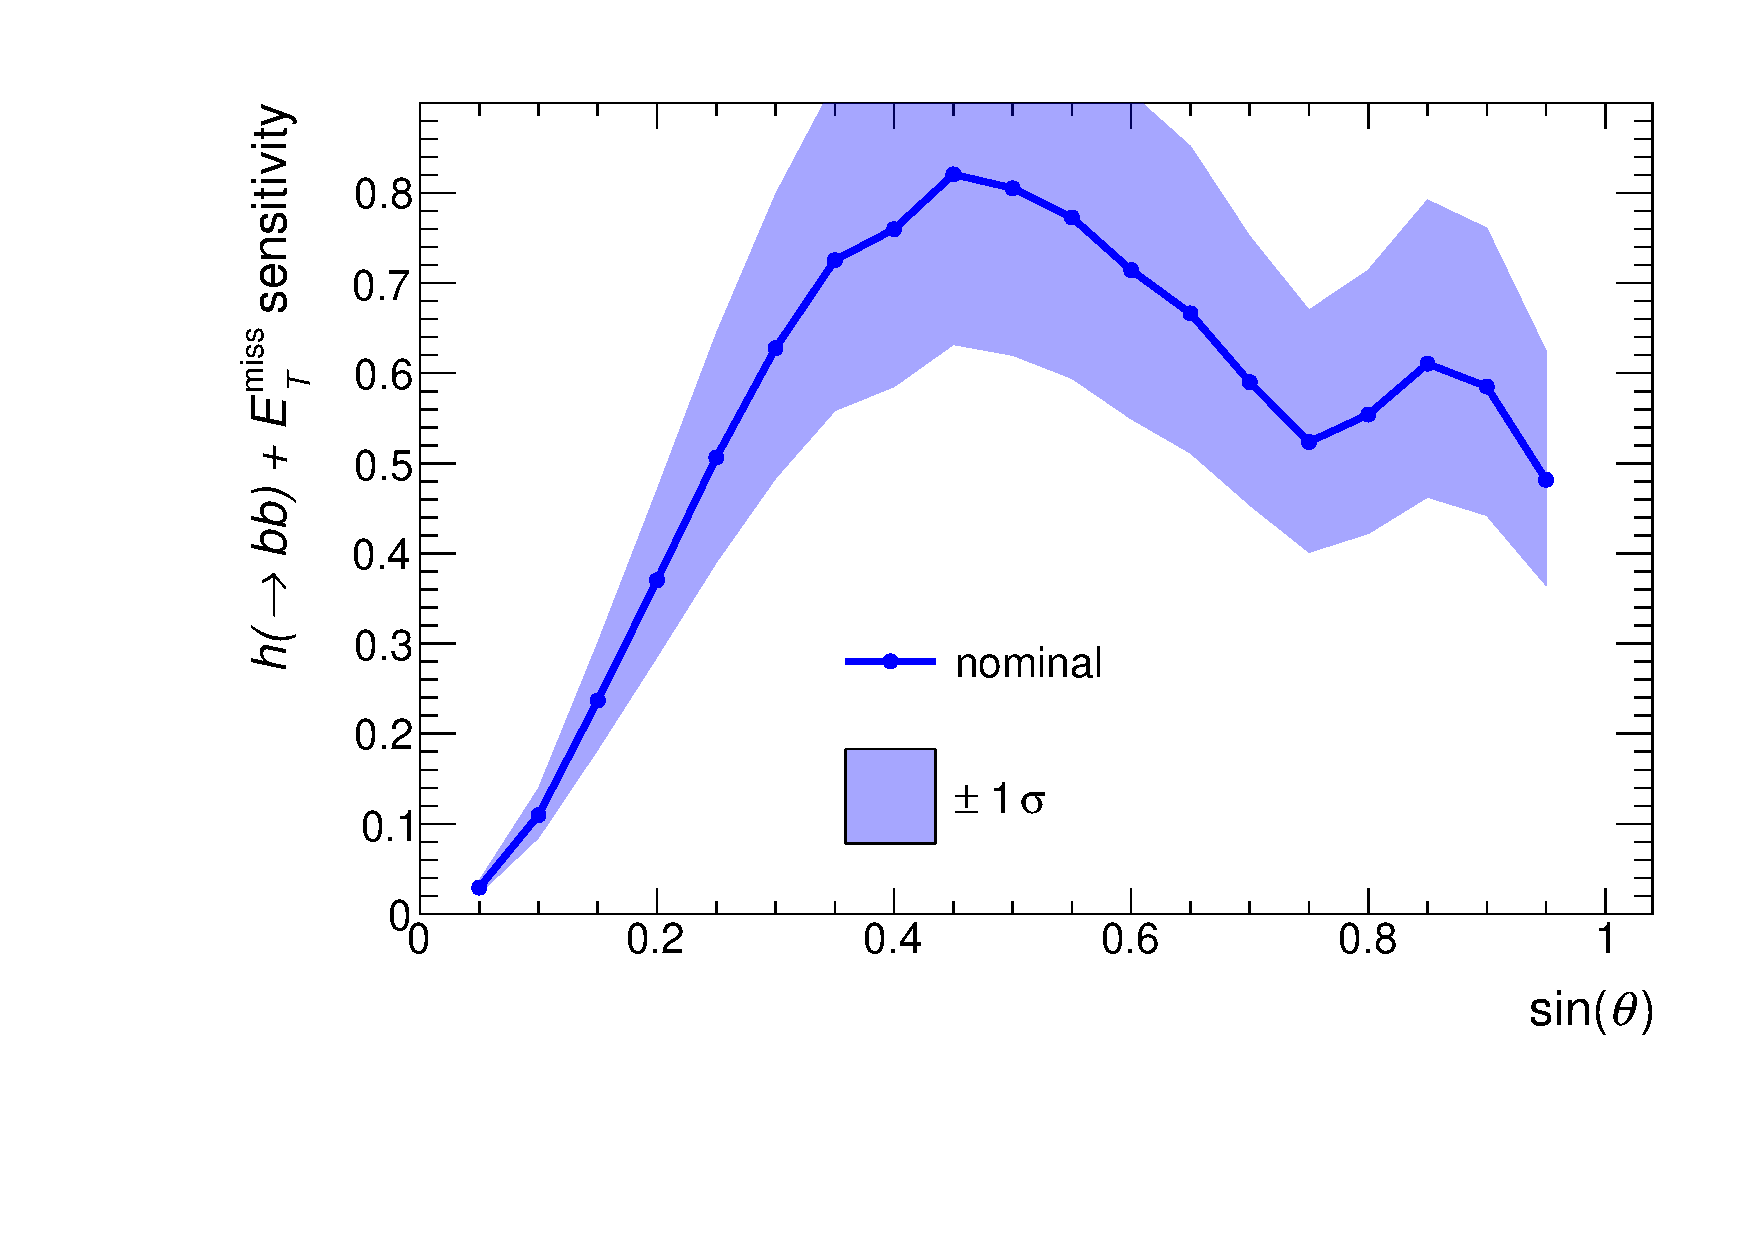
\includegraphics[width=0.49\textwidth]{texinputs/04_grid/figures/monoHbb_sinp_scan_2_sensi_1D.pdf}
%\caption[Sensitivity to $h\to bb + \MET$ signals with different $\sinp$, summed across $\MET$ bins]
%{
%Sum over all $\MET$-bins of the estimated signal sensitivity to $h\to bb + \MET$ events as a function of the pseudoscalar mixing parameter $\sinp$, for $\ma = 200~\GeV$ and $\mH=\mHc=\mA = 600$~GeV~(left) as well as $\ma = 350~\GeV$ and $\mH=\mHc=\mA = 1000$~GeV~(right). The remaining parameters take the values
%$\mDM = 10 $ GeV$, \tanb = 1,$ and $ \lap1 = \lap2 = \lam3 = 3 $.
%The sensitivity, defined in \autoref{eq:monoHbb_sensi}, as well as the uncertainty on the sensitivity (shaded blue) 
% are based on the limits with reduced model dependence from Ref.~\cite{Aaboud:2017yqz} and the uncertainties described therein. 
%}
%\label{fig:monoHbb_sensi_full_sinp}
%\end{figure}




%\begin{figure}[tbp]
%\centering
%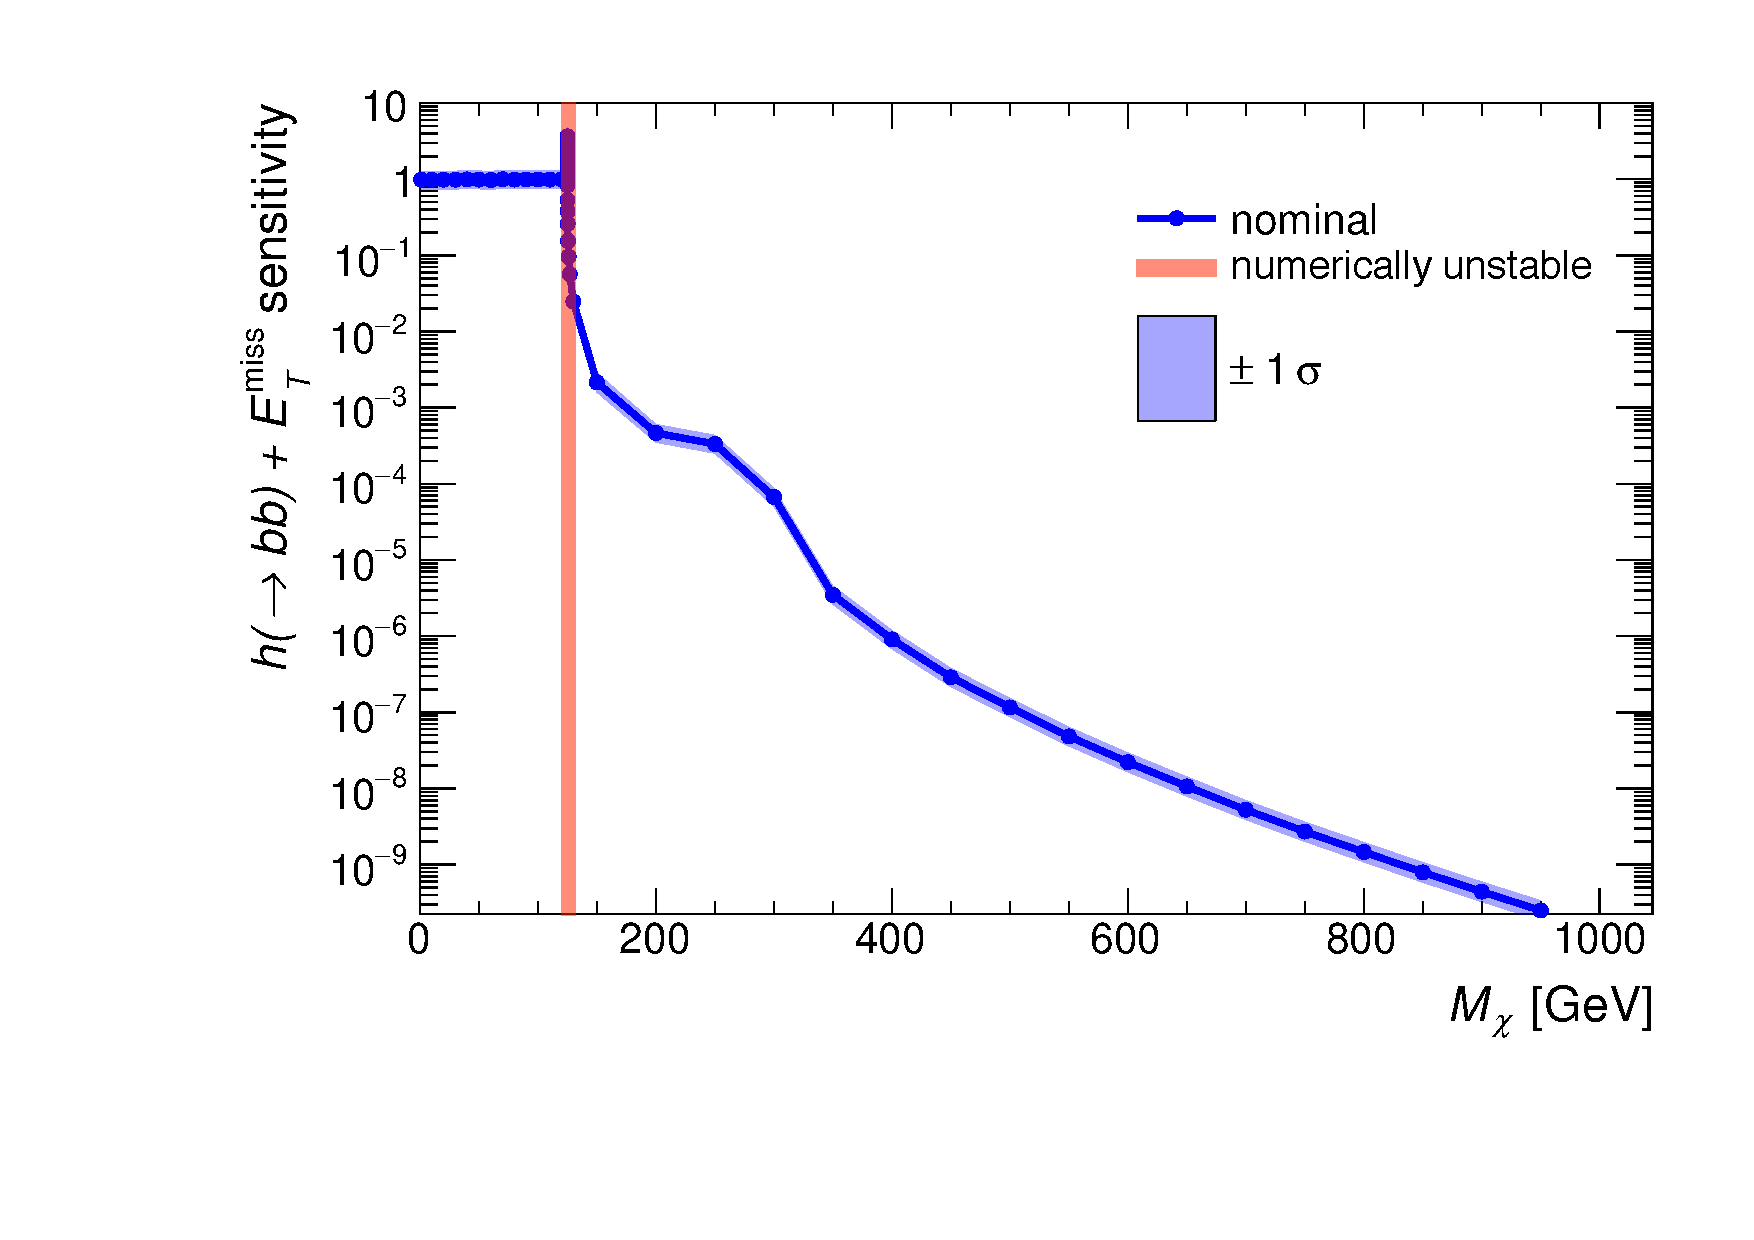
\includegraphics[width=0.7\textwidth]{texinputs/04_grid/figures/monoHbb_sensi_mDM_scan.pdf}
%\caption[Sensitivity to $h\to bb + \MET$ signals with different $\mDM$, summed across $\MET$ bins]
%{
%Sum over all $\MET$-bins of the estimated signal sensitivity to $h\to bb + \MET$ events as a function of the DM mass $\mDM$. 
%The sensitivity, defined in \autoref{eq:monoHbb_sensi}, as well as the uncertainty on the sensitivity (shaded blue)
%are based on the limits with reduced model dependence from Ref.~\cite{Aaboud:2017yqz} and the uncertainties described therein. 
%The remaining parameters take the values
%$ \ma = 250 $ GeV$, \mH=\mHc=\mA = 600$ GeV, $ \sinp = 0.35, \tanb = 1,$ and $ \lap1 = \lap2 = \lam3 = 3 $. 
%The sensitivity is constant below $\mDM < \ma/2$, and rapidly drops for $\mDM > \ma/2$. The sensitivity is resonantly enhanced for $\mDM = \ma/2$.}
%\label{fig:monoHbb_sensi_full_mDM}
%\end{figure}

%The sensitivity estimate of ATLAS and CMS to the \hdma scenario through the \monohbb signature is based on limits on anomalous production of 125 GeV Higgs bosons in association with \met with minimal model dependence~\cite{Aaboud:2017yqz}. The limits are translated to parton level and compared to parton-level simulations of the \hdma scenario for the sensitivity estimate. This approach avoids the simulation of the detector response, which requires a significant amount of computing resources, and more iterations and refinements of the signal grid can be performed. 

%The limits with minimal model dependence are provided in terms of the detector-level cross section of $\monohbb$ events $\sigma_{i}^{\mathrm{obs},\,\monohbb}$ as a function of \met in four bins $i=1,...4$~\cite{Aaboud:2017yqz}. 
%To compare these values to the simulation results at parton level, 
%an estimate of the detection efficiency $\varepsilon$ times the kinematic acceptance $\mathcal{A}$ of the event selections of the analysis is used for each of the four $\MET$ bins.
%%This estimate is provided as one $(\mathcal{A\times\varepsilon})$ value for each of the four $\MET$ bins. 
%Thus, the $(\mathcal{A}\times\varepsilon)_i$ figure represents the minimum probability
%that an event generated at parton level in a given $\MET$ bin $i$ is reconstructed in that same $\MET$ bin and passes all analysis selections.
%%The limits with minimal model dependence are provided separately for each of the four $\MET$ bins used in \cite{Aaboud:2017yqz}.
%%Thus, the simulated evebts are binned into those bins (\autoref{fig:monoHbb_xsec_bins_mA_ma}).
%Consequently, the cross section for \hdm production in the \hdma scenario at parton level $\sigma_{i}^{\mathrm{parton},\,\hdm}$ is calculated in the same $\MET$ bins as used in the \monohbb search. This starting point is shown in \autoref{fig:monoHbb_xsec_bins_mA_ma} using the scan in $(\mA,\ma)$ as a representative example. 
%In the next step, the sensitivity $\sens_i$ for each of the \met bins $i=1,...4$ is calculated as
%\begin{equation}
%\label{eq:monoHbb_sensi_i}
%\sens_i \equiv \frac{\sigma_{i}^{\mathrm{parton},\,\hdm} \times \mathcal{B}^{\mathrm{SM},\,h\to bb} \times (\mathcal{A\times\varepsilon})_{i} }
%{\sigma_{i}^{\mathrm{obs},\,\monohbb}}\,,
%\end{equation}
%where $\mathcal{B}^{\mathrm{SM},\,h\to bb}$ is the $h\to bb$ branching ratio predicted by the SM for the 125~GeV Higgs boson. A representative example for this step is given in \autoref{fig:monoHbb_sensi_bins_mA_ma} for the scan in $(\mA,\ma)$.  A particular point in the $(\mA,\ma)$ parameter parameter space is excluded if $\sens_i \geq 1$. Finally, to obtain a single estimate for the total sensitivity $\senstot$ using all four $\MET$ bins, their individual contributions from \autoref{eq:monoHbb_sensi_i} are summed over\footnote{
%This choice is made because the individual per-bin sensitivities follow a logarithmic metric, and because a model will typically populate several \met bins at a time. This implies that there could be models where $\sens_i<1$ in every bin, yet the sum from \autoref{eq:monoHbb_sensi} is $>1$.
%Therefore, for a rigorous exclusion of a model based on the limits with minimal model dependence, the preferred approach would be to consider only the most sensitive bin for the exclusion.
%}:
%\begin{equation}
%\label{eq:monoHbb_sensi}
%\senstot \equiv \sum_{i\in\met~\mathrm{bins}} \sens_i\,.
%\end{equation}
%The resulting $\senstot$ is shown in \autoref{fig:monoHbb_sensi_full_mA_ma} for the example of the $(\mA,\ma)$ scan.


%The scan of the sensitivity in the sense of \autoref{eq:monoHbb_sensi} in the $(\ma,\mA)$ plane is shown in \autoref{fig:monoHbb_sensi_full_mA_ma}.
%The sensitivity decreases with increasing $\mA = \mH = \mHc$ for $\mA \geq 1$~TeV because the fraction of resonant signal events drops. 
%This drop is caused by increasingly large $\Gamma_A$, 
%which allows for an increasing fraction of non-resonant signal events, driven by events with very off-shell $A$. % ref ggF-> A -> ah feynman graph
%%Non-resonant signal events have soft $\MET$ and thus the search is less sensitive to them, since the minimum accepted $\MET$ is $\MET \geq 150$ GeV.
%Near the mass diagonal $\ma = \mA$, there is little to no sensitivity. 
%This is because the Jacobian peak moves to low $\MET$ for a small mass splitting $|\mA - \ma|$
%(\autoref{eq:monoH_peak_met}, \autoref{fig:monoHbb_mA_scan_met}, and \autoref{fig:monoHbb_ma_scan_met}).
%Beyond this, the coupling $g_{Aah}$ is small when all Higgs bosons are nearly degenerate in mass, cf.~Equation~4.12 in Ref.~\cite{Bauer:2017ota}, %ref to eq.in theory part(?)
%resulting in a small total cross section and therefore further decrease in sensitivity.
%The sensitivity above the mass diagonal, $\mA > \ma$, is larger than below the mass diagonal.
%Two parameter choices cause this asymmetry:
%\begin{enumerate}
%\item 
%$\mA = \mH = \mHc$, i.e., the neutral and charged $CP$-even scalars have low masses below the diagonal, but high masses above it, introducing an asymmetry.
%Another effect can be seen in \autoref{fig:monoHbb_mH_scan_met}: values of  $\mH = \mHc$ below the mass of the higher-mass pseudoscalar (in this case $A$)
%give a reduced total cross section and a lower fraction of resonant signal events. Both effects reduce sensitivity;
%\item 
%$\sinp = 0.35 \neq 1/\sqrt{2}$, i.e. the mixing between the pseudoscalars $A$ and $a$ is asymmetric. 
%$A$ couples more strongly to SM particles than $a$, and vice versa for the couplings to the DM fermion $\chi$.
%So the situation below the diagonal corresponds to the case of $\sinp = \sqrt{1-0.35^2} \approx 0.938$ and $\mA > \ma$. 
%As can be seen in \autoref{fig:monoHbb_sinp_scan_mA600_ma200_met},
%this \sinp configuration has a higher fraction of non-resonant signal events with low \met, and correspondingly a lower sensitivity is found in \autoref{fig:monoHbb_sensi_full_sinp}.
%\end{enumerate}
%
%The scan of the sensitivity in the  $(\ma,\tanb)$ plane is shown in  \autoref{fig:monoHbb_sensi_full_ma_tanb}. 
%At very low $\tanb$, the Yukawa coupling to top quarks is large, and most of the signal events come from non-resonant processes, as can be seen from \autoref{fig:monoHbb_tanb_scan_met}. % ref to tanb met scan
%The non-resonant processes are characterised by soft $\MET$, which lowers the kinematic acceptance and reduces the sensitivity of the search.
%For higher $\tanb$, the fraction of resonant events increases due to the reduced top Yukawa coupling, resulting in an increase of sensitivity.
%However, reducing the top Yukawa coupling also reduces the total production cross section. 
%This effect is sub-dominant below $\tanb \approx 1.2$, and the sensitivity increases with $\tanb$. 
%But above $\tanb \approx 1.2$, the sensitivity loss due to reduced cross section outpaces the sensitivity gain due to a more resonant signal.
%Overall, the search gets less sensitive with increasing $\tanb$ above $\tanb \approx 1.2$.
%At very high $\tanb$ ($\geq 10$), this trend is reversed again because the $\tanb$ enhancement\footnote{The \hdma scenario assumes a Yukawa sector of type II.} of the 
%coupling to $b$-quarks compensates for the small $b$-quark mass.
%At this point $bb$ initiated processes start to dominate the production cross section and drive the increase in sensitivity.
%
%The sensitivity to models with varying $\sinp$ is shown in \autoref{fig:monoHbb_sensi_full_sinp}.
%The sensitivity vanishes at $\sinp=0$ and $\sinp=1$, since those values correspond to no mixing between $A$ and $a$, and thus no connection between the SM and the dark sector. 
%For its intermediate values, the $\sinp$ parameter influences the couplings of the pseudoscalars to DM as well as to SM fermions, 
%and also the coupling strength of trilinear scalar vertices such as $g_{Aah}$~\cite{Bauer:2017ota}. 
%Increasing the couplings increases the total cross section. 
%However, increasing some couplings can also increase $\Gamma_A$ and thereby decrease the resonant fraction of signal events and the sensitivity.
%The upshot of this is that there can be more than one local maximum in the sensitivity curve, as shown the right panel of~\autoref{fig:monoHbb_sensi_full_sinp}. 
%The precise dependence of the sensitivity on \sinp depends on the precise interplay of the couplings.
%Because the couplings depend on all other model parameters including all the Higgs masses, 
%tuning the $\sinp$ of a parameter scan to the sensitivity in a single point can lead to sub-optimal sensitivity in other points.
%
%The sensitivity to models with varying $\mDM$ is shown in  \autoref{fig:monoHbb_sensi_full_mDM}.
%Below the threshold of $\mDM < \ma/2$, the sensitivity is constant since the $\MET$ distribution and the total signal cross section remain invariant, as demonstrated in \autoref{fig:monoHbb_mDM_scan_met}.
%At threshold, the sensitivity is enhanced because the partial width for $ a \to \chi \chi $ is enhanced, 
%increasing the signal cross section.
%Above threshold, the sensitivity drops rapidly because $\mDM > \ma/2$ requires an off-shell $a^{\star} \to \chi\chi$ decay, which is strongly suppressed by the typically  narrow width of $a$. 
%The width of $a$ is substantially reduced once $a\to \chi \chi$ is kinematically inaccessible, 
%as $\Gamma_{a\to \chi \chi}$ is a large contribution to the total width of $a$ for $\mDM \leq \ma/2$ \cite{Bauer:2017ota}.
%There is a slight increase in sensitivity for $\mDM \approx \mA/2$ when the $A\to \chi\chi$ decay hits its kinematic threshold, yet the absolute sensitivity remains negligible.
